\documentclass{beamer}

\usepackage{hyperref}
\usepackage{amsmath}
\usepackage{amsfonts}
\usepackage[ruled]{algorithm}
\usepackage{algpseudocode}
\usepackage{graphicx}
\usepackage{minted}

\newcommand {\I} {\ensuremath {\mathbf{1\hspace{-5.5pt}1}}}
\renewcommand{\vec}[1]{\ensuremath{\boldsymbol{#1}}}

\title{Design and Implementation of\\Anglican Probabilistic Programming Language}
\author{David Tolpin \and Jan Willem van de Meent \and Hongseok Yang \and Frank Wood}
  
\AtBeginSection[]
{
  \begin{frame}<beamer>
    \frametitle{Outline}
    \tableofcontents[currentsection]
  \end{frame}
}

\begin{document}


\begin{frame}
\titlepage
\vfill
\center
\url{https://bitbucket.org/probprog/anglican-white-paper}\\
\url{https://bitbucket.org/probprog/anglican} \\
\url{http://www.robots.ox.ac.uk/~fwood/anglican/index.html}

\end{frame}

\section{Motivation}

\begin{frame}{Intuition}
    \textbf{Probabilistic program:}
\begin{itemize}
\item A program with random computations.
\item Distributions are conditioned by `observations'.
\item Values of certain expressions are `predicted' --- \textbf{the output}.
\end{itemize}

Can be written in any language (extended by \texttt{sample} and \texttt{observe}).
\end{frame}

\begin{frame}[fragile]{Example: Model Selection}
\begin{minted}[linenos, fontsize=\small]{clojure}
(let [;; Guessing a distribution
      dist (sample (categorical
                     [[normal 1] [gamma 1]
                      [uniform-continuous 1]
                      [uniform-discrete 1]]))
      a (sample (gamma 1 1))
      b (sample (gamma 1 1))
      d (dist a b)]
  ;; Observing samples from the distribution
  (loop [data data]
    (when (seq data)
      (let [[x & data] data]
        (observe d x))
      (recur data)))
  ;; Predicting a, b and the distribution
  (predict :a a) 
  (predict :b b)
  (predict :d d))
\end{minted}
\end{frame}

\begin{frame}{More examples}
    \begin{itemize}
        \item \textit{Intruder detection} --- 
            given a log of \textbf{times} and \textbf{amounts} of
            payments in a bank account, how likely that the baccount was
            compromised?
        \pause
        \item \textit{Counterfactual reasoning} --- There are
            \textbf{two routes} from Jerusalem to Tel Aviv:
            1 and 443.  Based on traffic reports, I chose route
            1 and was late. Would I arrive on time If I chose 443
            instead?
        \pause 
        \item \textit{(Due to Stuart Russell)} If you observe that a
            student GPA is exactly 4.0 in a model of
            transcripts of students from the USA (GPA's from
            0.0 to 4.0) and India (GPA's from 0.0 to
            10.0) what is the probability that the student
            is from India? 
    \end{itemize}
\end{frame}

\begin{frame}{Inference Objective}
\begin{itemize}
\item Suggest \textbf{most probable explanation} (MPE) - most likely assignment
  for all non-evidence variable given evidence.
  \pause
\item Approximately \textbf{compute integral} of the
  form $$\Phi=\int_{-\infty}^{\infty} \varphi(x)p(x) dx$$
  \pause
\item Continuously and \textbf{infinitely generate a sequence of samples} drawn
  from the distribution of the output expression --- so that someone
  else puts it in good use (vague but common). $\checkmark$
\end{itemize}
\end{frame}

\begin{frame}{Example: Inference Results}
  \begin{figure}[H]
      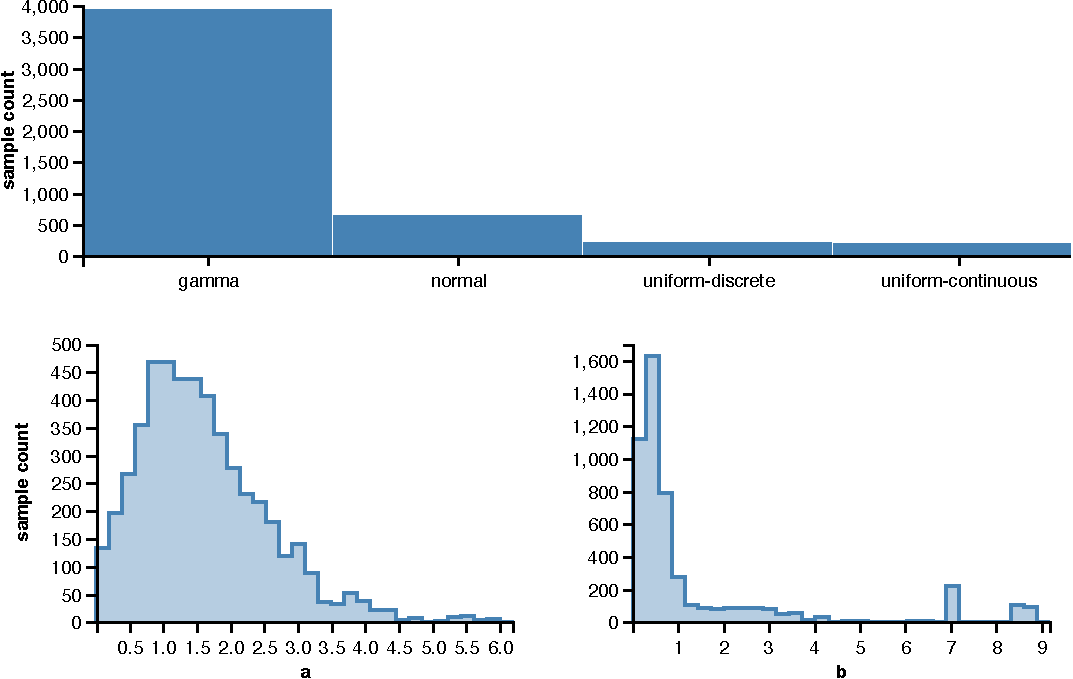
\includegraphics[scale=0.6]{models-results.pdf}
  \end{figure}
\end{frame}

\begin{frame}{Importance Sampling}
    \begin{algorithmic}
        \Loop
            \State Run program, computing weight based on observations.
            \State Output result and weight.
        \EndLoop
    \end{algorithmic}
    \begin{itemize}
        \item[] 
         \item Simple --- good.
         \item Slow convergence (unless one knows the answer) --- bad.
     \end{itemize}
     \vfill
     Can we do better?
\end{frame}

\begin{frame}{Lightweight Metropolis-Hastings (LMH)}
\begin{algorithmic}
    \State Run program once, remembering random choices.
    \Loop
         \State Uniformly select one random choice.
         \State Propose a new value for the choice.
         \State Re-run the program.
         \State Accept or reject with MH probability.
         \State Output result.
    \EndLoop
\end{algorithmic}
\vfill
Can we do better?
\begin{itemize}
    \item Particle methods
    \item Variational inference
    \item ...
\end{itemize}
\end{frame}

\begin{frame}{Why functional?}
    We want a functional language because an inference algorithm
    controls the execution:
    \begin{itemize}
        \item A program is run many (often many hundreds of
            thousands) of times (with almost any algorithm).
        \item A program must be partially re-executed multiple
            times from different positions (particle methods).
        \item We want to reason about the distribution defined
            by the program.
    \end{itemize}
\end{frame}

\begin{frame}{Why Closure?}
\begin{itemize}
    \item Runs on JVM --- easy deployment and access to libraries.
        \pause
    \item A Lisp --- we (ab)use the macro facility.
        \pause
    \item Church (\url{https://en.wikipedia.org/wiki/Church_(programming_language)}) is derived from Scheme.
\end{itemize}
\pause
Others use:
    \begin{itemize}
        \item Scheme --- (Church, Venture).
        \item Scala --- Figaro.
        \item Haskell --- Hakaru, Model-Bayes.
        \item ...
    \end{itemize}
    \pause
    As well as Python, C\#,  and other languages.
\end{frame}

\section{Design Outline}

\begin{frame}{Anglican and Clojure}
    One language on top of (or besides) another:
    \begin{itemize}
        \item Interpeter.
        \item Source-to-source compiler.
        \item Integrated language. $\checkmark$
    \end{itemize}
    \pause
    \bigskip
    Integrated language
    \begin{itemize}
        \item either extends the syntax of the host language;
        \item or changes the semantics of the host language
            constructs $\checkmark$.
    \end{itemize}
    \pause
    \bigskip
    Anglican is 
    \begin{itemize}
        \item Integrated with Clojure.
        \item Shares syntax.
        \item Alters operational semantics.
    \end{itemize}
\end{frame}

\begin{frame}{Design challenges and choices}
\begin{itemize}
    \item Anglican syntax: Clojure + probabilistic constructs.
		\begin{itemize}
			\item Subset of Clojure.
			\item Special forms \texttt{sample} and \texttt{observe}.
			\item Macros to delimit Anglican code within a Clojure program.
		\end{itemize}
		\pause
		\bigskip
    \item Source-to-source compilation of Anglican into Clojure.
		\begin{itemize}
			\item CPS Transformation, with some tricks.
			\item Transparent use of Clojure functions from Anglican.
		\end{itemize}
		\pause
		\bigskip
    \item Inference algorithms.
		\begin{itemize}
            \item Required to run an Anglican program.
			\item Step in at checkpoints (\texttt{sample} and \texttt{observe}).
			\item Execute programs by calling continuations repeatedly.
		\end{itemize}
\end{itemize}
\end{frame}

\begin{frame}{The language}
    A subset of Clojure, wrapped inside \texttt{defquery}:
    \begin{itemize}
        \item \texttt{if}, \texttt{when}, \texttt{cond},
            \texttt{case}, \texttt{let}, \texttt{and}, \texttt{or},
            \texttt{fn}. 
        \item Vector destructuring in bindings of \texttt{let} and \texttt{fn}.
        \item Compound literals for vectors, hash maps, and sets.
        \item \texttt{loop}/\texttt{recur} --- a convenience.
    \end{itemize}
    \bigskip
    Core library:
    \begin{itemize}
        \item All of Clojure core library, except for
            higher-order functions.
        \item  \texttt{map}, \texttt{reduce},
\texttt{filter}, \texttt{some}, \texttt{repeatedly},
\texttt{comp}, \texttt{partial}.
    \end{itemize}
    \bigskip
    Any Clojure function can be called from Anglican.
\end{frame}

\begin{frame}[fragile]{Macro-based compilation}
    Anglican code macro-compiled into Clojure:
    \begin{minipage}{0.48\textwidth}
\begin{minted}[linenos, fontsize=\scriptsize]{clojure}
(loop [data data]
  (if (seq data)
    (let [[x & data] data]
      (observe (gamma a b) x)
      (recur data))
    (predict :a a)))
\end{minted}
    \end{minipage}
    \begin{minipage}{0.44\textwidth}
    \vspace{2em}
\begin{minted}[linenos, fontsize=\scriptsize]{clojure}
(fn loop [C23151 state data]
   (if (seq data)
     (let [[x & data] data]
       (->observe 'O23153 (gamma a b) x
         (fn do23152 [_ state]
           (loop C23151 state data))
         state))
     (fn []
       (C23151
         nil
         (add-predict state :a a)))))
\end{minted}
    \end{minipage}
\end{frame}

\section{Implementation Highlights}

\begin{frame}[fragile]{Probabilistic forms}
    Two \textbf{probabilistic} forms:
    \begin{itemize}
        \item \texttt{sample} --- draws a value from a
            distribution;
        \item \texttt{observe} --- conditions the \textit{a
            posteriori} distribution by observing a value from a
            distribution.
    \end{itemize}
    \bigskip
    This is where the inference algorithm steps in:
\begin{minted}[fontsize=\small]{clojure}
=> (cps-of-expression '(sample dist) 'cont)
(->sample dist cont $state)

=> (cps-of-expression '(observe dist val) 'cont)
(->observe dist val cont $state)
\end{minted}
\end{frame}

\begin{frame}[fragile]{Memoization}
Memoization of random choice:
\begin{itemize}
    \item A person has a random eye color.
    \item But the \textit{same} person has a fixed eye color.
\end{itemize}
\begin{minted}[linenos, fontsize=\small]{clojure}
(let [eye-color (mem (fn [person] 
                       (sample 
                         (categorical
                           ['brown 0.5]
                           ['green 0.5]))))]
  (if (not= (eye-color 'bill) (eye-color 'john))
    (predict (eye-color 'bill))
    (predict (eye-color 'john))))
\end{minted}
\end{frame}

\begin{frame}[fragile]{Compiling a memoized function}
    \vspace{-2em}
    \begin{minipage}{0.38\textwidth}
\begin{minted}[linenos, fontsize=\scriptsize]{clojure}
(mem (fn [person] ...))
\end{minted}
    \end{minipage}
    \begin{minipage}{0.52\textwidth}
    \vspace{2em}
\begin{minted}[linenos, fontsize=\scriptsize]{clojure}
(fn []
 (cont
  ;; every memoization gets a unique key  
  (let [M23145 (gensym "M")]
   (fn [C23144 $state & P23147]
    (if (in-mem? $state M23145 P23147)
     ;; previously memoized result
     (fn []
       (C23144
         (get-mem $state M23145 P23147)
         $state))
     ;; new computation
     (clojure.core/apply
      (fn [C23150 $state person]
        (fn [] (C23150 ... $state)))
      ;; memoize result in state
      (fn [V23146 $state]
       (fn []
        (C23144
          V23146
          (set-mem $state M23145 P23147 V23146))))
      $state
      P23147))))
  $state))
\end{minted}
    \end{minipage}
\end{frame}

\begin{frame}[fragile]{Managing stack size}
    \begin{itemize}
        \item Clojure does not support tail-call optimization (TCO).
        \item Under CPS transformation the stack will explode.
            \pause
        \item Anglican uses \textit{trampolining}: every continuation
            call is wrapped into a \textit{thunk}.
    \end{itemize}

    The thunk is returned ...

    \begin{minipage}{0.48\textwidth}
\begin{minted}[linenos, fontsize=\scriptsize]{clojure}
    (fn [x y] (+ x y))
\end{minted}
    \end{minipage}
    \begin{minipage}{0.48\textwidth}
        \vspace{0.5em}
\begin{minted}[linenos, fontsize=\scriptsize]{clojure}
    (fn [cont $state x y] 
      (fn []
        (cont (+ x y) $state)))
\end{minted}
      \vspace{0.5em}
    \end{minipage}

    ... and  called by \texttt{trampoline}:

\begin{minted}[linenos, fontsize=\small]{clojure}
        (defn exec
          [algorithm prog value state]
          (loop [step (trampoline prog value state)]
            (let [next (checkpoint algorithm step)]
              (if (fn? next)
                (recur (trampoline next))
                next))))
\end{minted}

\end{frame}

\section{Inference Algorithms}

\begin{frame}[fragile]{Importance sampling}

Importance sampling is the simplest:
\begin{minted}[linenos, fontsize=\small]{clojure}
(defmethod infer :importance [_ prog value & {}]
  (letfn
    [(sample-seq []
       (lazy-seq
         (cons
           (:state (exec ::algorithm prog value
                         initial-state))
           (sample-seq))))]
    (sample-seq)))
\end{minted}
Default checkpoint handlers are called:
\begin{minted}[linenos, fontsize=\scriptsize]{clojure}
(defmethod checkpoint [::algorithm anglican.trap.observe] [_ obs]
  #((:cont obs) nil (add-log-weight (:state obs)
                                    (observe* (:dist obs) (:value obs)))))

(defmethod checkpoint [::algorithm anglican.trap.sample] [_ smp]
  #((:cont smp) (sample* (:dist smp)) (:state smp)))
\end{minted}
\end{frame}

\begin{frame}{Other inference algorithms}
    \begin{itemize}
        \item Implement \texttt{infer}.
        \item Redefine one or both checkpoints.
        \item An average implementation is $\approx 150$ lines of source
            code.
        \item A dozen different inference algorithms are in the
            code base.
        \item Half of them are really useful.
    \end{itemize}
\end{frame}

\begin{frame}{Recap}
    \begin{itemize}
        \item Anglican is integrated with Clojure.
        \item Shares syntax but alters semantics.
        \item Macro-compiled.
        \item Efficient.
        \item Makes implementing AND using inference easy.
    \end{itemize}
\end{frame}

\begin{frame}
    \LARGE
    \center
    Thank you!\\Questions?
\end{frame}

\end{document}
